\documentclass[11pt,a4paper]{scrartcl}

%% ============================================================
%%  PACKAGES
%% ============================================================
\usepackage[T1]{fontenc}
\usepackage[utf8]{inputenc}
\usepackage{lmodern}
\usepackage{microtype}
\usepackage[top=22mm,bottom=24mm,left=22mm,right=22mm]{geometry}
\usepackage[table]{xcolor}
\usepackage{amsmath,amssymb}
\usepackage{graphicx}
\usepackage{array}
\usepackage{booktabs}
\usepackage{tabularx}
\usepackage{colortbl}
\usepackage{multirow}
\usepackage{enumitem}
\usepackage{parskip}
\usepackage{setspace}
\usepackage{mdframed}
\usepackage{tikz}
\usepackage{pgfornament}
\usepackage[most]{tcolorbox}
\usepackage{fontawesome5}
\usepackage{hyperref}
\usepackage{fancyhdr}
\usepackage{lastpage}
\usepackage{soul}
\usepackage{dashrule}
\usepackage{ifthen}
\usepackage{calc}
\usepackage{etoolbox}
\usepackage{ragged2e}

\usetikzlibrary{positioning,calc,shapes.geometric,decorations.pathmorphing,backgrounds,patterns}

%% ============================================================
%%  COLOURS
%% ============================================================
\definecolor{NavyDeep}{HTML}{0D2545}
\definecolor{TealAccent}{HTML}{1A7A8A}
\definecolor{WarmGold}{HTML}{C8962E}
\definecolor{PaperCream}{HTML}{F7F4EF}
\definecolor{SlateGray}{HTML}{4A5568}
\definecolor{LightRule}{HTML}{CBD5E0}
\definecolor{AlertRed}{HTML}{C53030}
\definecolor{AlertRedBg}{HTML}{FFF5F5}
\definecolor{FieldBg}{HTML}{EEF2F7}
\definecolor{SuccessGreen}{HTML}{276749}
\definecolor{SuccessGreenBg}{HTML}{F0FFF4}
\definecolor{HeaderBg}{HTML}{0D2545}
\definecolor{SubheadBg}{HTML}{1A3A5C}

%% ============================================================
%%  HYPERREF
%% ============================================================
\hypersetup{
  colorlinks=false,
  hidelinks,
  pdfauthor={Meridian Pharmacovigilance Unit},
  pdftitle={Adverse Event Report -- MPN-AE-2024-00847},
  pdfsubject={Pharmacovigilance / Drug Safety},
}

%% ============================================================
%%  FONTS (pdflatex)
%% ============================================================
\usepackage{helvet}
\renewcommand{\familydefault}{\sfdefault}

%% ============================================================
%%  HEADER / FOOTER
%% ============================================================
\pagestyle{fancy}
\fancyhf{}
\renewcommand{\headrulewidth}{0pt}
\renewcommand{\footrulewidth}{0pt}

\fancyhead[L]{%
  \begin{tikzpicture}[remember picture, overlay]
    \fill[NavyDeep] (current page.north west)
      rectangle ([yshift=-14mm]current page.north east);
  \end{tikzpicture}%
  \raisebox{-4pt}{\color{white}\small\textbf{MERIDIAN PHARMACOVIGILANCE UNIT}}%
}
\fancyhead[R]{%
  \color{white}\small\textbf{Adverse Event Report}%
  \quad\textcolor{WarmGold}{\rule[-1pt]{0.5pt}{9pt}}\quad%
  \color{white}\small MPN-AE-2024-00847%
}

\fancyfoot[L]{\color{SlateGray}\footnotesize\textit{Confidential -- For Regulatory Use Only}}
\fancyfoot[C]{\color{SlateGray}\footnotesize Page \thepage\ of \pageref{LastPage}}
\fancyfoot[R]{\color{SlateGray}\footnotesize \textit{Version 1.0 \textbar{} 2024-09-15}}

%% ============================================================
%%  CUSTOM TCOLORBOX STYLES
%% ============================================================
\tcbuselibrary{skins,breakable,listings}

% Section header box
\newtcolorbox{sectionbox}[2][]{
  enhanced,
  arc=3pt,
  outer arc=3pt,
  colback=NavyDeep,
  colframe=NavyDeep,
  fonttitle=\bfseries\color{white}\normalsize,
  coltitle=white,
  title={\faChevronRight\quad #2},
  top=3pt, bottom=3pt, left=8pt, right=8pt,
  boxrule=0pt,
  #1
}

% Field box (light blue bg)
\newtcolorbox{fieldbox}[1][]{
  enhanced,
  arc=2pt, outer arc=2pt,
  colback=FieldBg,
  colframe=LightRule,
  boxrule=0.6pt,
  top=4pt, bottom=4pt, left=6pt, right=6pt,
  #1
}

% Alert box
\newtcolorbox{alertbox}[2][]{
  enhanced,
  arc=3pt, outer arc=3pt,
  colback=AlertRedBg,
  colframe=AlertRed,
  fonttitle=\bfseries\color{AlertRed}\small,
  coltitle=AlertRed,
  title={#2},
  boxrule=1pt,
  top=4pt, bottom=4pt, left=8pt, right=8pt,
  #1
}

% Info note box
\newtcolorbox{notebox}[1][]{
  enhanced,
  arc=2pt, outer arc=2pt,
  colback=SuccessGreenBg,
  colframe=SuccessGreen,
  boxrule=0.8pt,
  top=3pt, bottom=3pt, left=6pt, right=6pt,
  #1
}

% Subsection label box
\newtcolorbox{subsecbox}[2][]{
  enhanced,
  arc=2pt, outer arc=2pt,
  colback=SubheadBg,
  colframe=SubheadBg,
  fonttitle=\bfseries\color{white}\small,
  coltitle=white,
  title={#2},
  boxrule=0pt,
  top=2pt, bottom=2pt, left=6pt, right=6pt,
  #1
}

% Signature box
\newtcolorbox{sigbox}[1][]{
  enhanced,
  arc=2pt, outer arc=2pt,
  colback=PaperCream,
  colframe=LightRule,
  boxrule=0.6pt,
  top=10pt, bottom=10pt, left=10pt, right=10pt,
  #1
}

%% ============================================================
%%  UTILITY COMMANDS
%% ============================================================
\newcommand{\fieldlabel}[1]{%
  \textcolor{SlateGray}{\footnotesize\textbf{#1}}%
}
\newcommand{\fieldvalue}[1]{%
  {\normalsize #1}%
}
\newcommand{\sectionrule}{%
  \vspace{1pt}%
  {\color{WarmGold}\rule{\linewidth}{1.5pt}}%
  \vspace{4pt}%
}
\newcommand{\thinrule}{%
  {\color{LightRule}\rule{\linewidth}{0.5pt}}%
}
\newcommand{\severity}[1]{%
  \begin{tikzpicture}[baseline=-2pt]
    \fill[AlertRed] (0,0) circle (5pt);
    \node[white,font=\tiny\bfseries] at (0,0) {#1};
  \end{tikzpicture}%
}
\newcommand{\checkbox}[1]{%
  \ifthenelse{\equal{#1}{checked}}{%
    \tikz[baseline=-1pt]{\fill[TealAccent] (0,0) rectangle (8pt,8pt);
    \draw[white,line width=1.2pt] (1.5pt,4pt)--(3.5pt,6.5pt)--(6.5pt,1.5pt);}%
  }{%
    \tikz[baseline=-1pt]{\draw[SlateGray,line width=0.7pt] (0,0) rectangle (8pt,8pt);}%
  }%
}

%% ============================================================
%%  COLUMN TYPES
%% ============================================================
\newcolumntype{L}[1]{>{\RaggedRight\arraybackslash}p{#1}}
\newcolumntype{C}[1]{>{\Centering\arraybackslash}p{#1}}
\newcolumntype{R}[1]{>{\RaggedLeft\arraybackslash}p{#1}}

%% ============================================================
%%  DOCUMENT
%% ============================================================
\begin{document}

\setlength{\parskip}{6pt}

%% ============================================================
%%  TITLE BLOCK
%% ============================================================
\vspace*{4mm}

\begin{tikzpicture}[remember picture]
  \node[inner sep=0pt] (titleblock) {%
    \begin{minipage}{\linewidth}
      \begin{tcolorbox}[
        enhanced,
        arc=4pt, outer arc=4pt,
        colback=PaperCream,
        colframe=NavyDeep,
        boxrule=2pt,
        top=10pt, bottom=10pt, left=14pt, right=14pt,
      ]
        \begin{minipage}[c]{0.60\linewidth}
          {\color{NavyDeep}\LARGE\bfseries Pharmacovigilance}\\[2pt]
          {\color{TealAccent}\large\bfseries Adverse Event Report}\\[4pt]
          {\color{SlateGray}\small\textit{Individual Case Safety Report (ICSR)}}
        \end{minipage}%
        \hfill%
        \begin{minipage}[c]{0.36\linewidth}
          \RaggedLeft
          \begin{tabular}{@{}r@{}}
            \color{SlateGray}\footnotesize Report No.\\
            {\color{NavyDeep}\normalsize\bfseries MPN-AE-2024-00847}\\[4pt]
            \color{SlateGray}\footnotesize Report Date\\
            {\color{NavyDeep}\normalsize\bfseries 15 September 2024}\\[4pt]
            \color{SlateGray}\footnotesize Classification\\
            \begin{tikzpicture}[baseline=-1pt]
              \fill[AlertRed] (0,0) rectangle (55pt,11pt);
              \node[white,font=\tiny\bfseries,inner sep=0pt] at (27.5pt,5.5pt) {SERIOUS -- EXPEDITED};
            \end{tikzpicture}
          \end{tabular}
        \end{minipage}
      \end{tcolorbox}
    \end{minipage}%
  };
\end{tikzpicture}

\vspace{4mm}

%% ============================================================
%%  SECTION 1: ADMINISTRATIVE INFORMATION
%% ============================================================
\begin{sectionbox}{\faBuilding\quad Section 1 \textbar{} Administrative Information}
\end{sectionbox}
\sectionrule

\begin{minipage}[t]{0.48\linewidth}
\fieldlabel{Reporting Organisation}\\
\fieldvalue{\textbf{Meridian Pharmaceutical Ltd.}}\\[1pt]
\fieldlabel{Department}\\
\fieldvalue{Global Drug Safety \& Pharmacovigilance}\\[1pt]
\fieldlabel{Address}\\
\fieldvalue{14 Synapse Plaza, Tower B, Floor 8\\
London EC2N 4AA, United Kingdom}\\[1pt]
\fieldlabel{EudraVigilance Registration No.}\\
\fieldvalue{EVMPD-GB-MPN-0041}
\end{minipage}%
\hfill%
\begin{minipage}[t]{0.48\linewidth}
\fieldlabel{Primary Contact -- Safety Officer}\\
\fieldvalue{\textbf{Dr. Helena Strauss, PharmD}}\\[1pt]
\fieldlabel{Direct Line}\\
\fieldvalue{+44 (0)20 7946 0182}\\[1pt]
\fieldlabel{Email}\\
\fieldvalue{h.strauss@meridian-pharma.fictional}\\[1pt]
\fieldlabel{Regulatory Submission Deadline}\\
\fieldvalue{\textbf{22 September 2024} \quad
  
\begin{tikzpicture}[baseline=-2pt]
    \draw[AlertRed,line width=1pt] (0,0) circle (5pt);
    \node[AlertRed,font=\tiny\bfseries] at (0,0) {!};
  \end{tikzpicture}
  \textcolor{AlertRed}{\footnotesize\bfseries Expedited 7-Day}}\\[1pt]
\fieldlabel{Worldwide Unique Case ID}\\
\fieldvalue{GB-MPN-2024-AE-847}
\end{minipage}

\vspace{3mm}
\thinrule
\vspace{2mm}

\noindent
\fieldlabel{Source Type:}\quad
\checkbox{checked}~\footnotesize Spontaneous Report\quad
\checkbox{}~\footnotesize Literature\quad
\checkbox{}~\footnotesize Clinical Trial\quad
\checkbox{}~\footnotesize Regulatory Authority\quad
\checkbox{}~\footnotesize Health Professional

\vspace{5mm}

%% ============================================================
%%  SECTION 2: PATIENT INFORMATION
%% ============================================================
\begin{sectionbox}{\faUser\quad Section 2 \textbar{} Patient Information}
\end{sectionbox}
\sectionrule

\begin{minipage}[t]{0.31\linewidth}
\fieldlabel{Patient Initials}\\
\fieldvalue{\textbf{R.K.T.}}\\[3pt]
\fieldlabel{Date of Birth}\\
\fieldvalue{12 March 1968}\\[3pt]
\fieldlabel{Age at Onset}\\
\fieldvalue{\textbf{56 years}}\\[3pt]
\fieldlabel{Sex}\\
\fieldvalue{Male}
\end{minipage}%
\hfill%
\begin{minipage}[t]{0.31\linewidth}
\fieldlabel{Weight}\\
\fieldvalue{82 kg}\\[3pt]
\fieldlabel{Height}\\
\fieldvalue{178 cm}\\[3pt]
\fieldlabel{BMI}\\
\fieldvalue{25.9 kg/m\textsuperscript{2}}\\[3pt]
\fieldlabel{Ethnicity (self-reported)}\\
\fieldvalue{Caucasian}
\end{minipage}%
\hfill%
\begin{minipage}[t]{0.31\linewidth}
\fieldlabel{Country of Occurrence}\\
\fieldvalue{United Kingdom}\\[3pt]
\fieldlabel{Reporting Physician}\\
\fieldvalue{\textbf{Dr. Marcus Okafor}}\\[3pt]
\fieldlabel{Institution}\\
\fieldvalue{Nexabridge General Hospital}\\[3pt]
\fieldlabel{Specialty}\\
\fieldvalue{Cardiology / Internal Medicine}
\end{minipage}

\vspace{4mm}

\begin{subsecbox}{Relevant Medical History \& Pre-existing Conditions}
\end{subsecbox}

\vspace{2mm}
\begin{tabular}{@{}L{0.28\linewidth}L{0.20\linewidth}L{0.22\linewidth}L{0.22\linewidth}@{}}
\toprule
\rowcolor{FieldBg}
\small\bfseries Condition & \small\bfseries ICD-10 & \small\bfseries Onset & \small\bfseries Status \\
\midrule
Type 2 Diabetes Mellitus & E11.9 & 2015 & Ongoing \\
\rowcolor{FieldBg}
Essential Hypertension & I10 & 2012 & Ongoing \\
Dyslipidaemia & E78.5 & 2018 & Ongoing \\
\rowcolor{FieldBg}
Stable Angina Pectoris & I20.8 & 2021 & Ongoing \\
Previous MI (inferior) & I21.1 & Jan 2022 & Resolved \\
\bottomrule
\end{tabular}

\vspace{4mm}

\begin{subsecbox}{Known Allergies \& Intolerances}
\end{subsecbox}

\vspace{2mm}
\begin{tabular}{@{}L{0.30\linewidth}L{0.28\linewidth}L{0.34\linewidth}@{}}
\toprule
\rowcolor{FieldBg}
\small\bfseries Substance & \small\bfseries Reaction Type & \small\bfseries Severity \\
\midrule
Penicillin (all classes) & Anaphylaxis & Life-threatening \\
\rowcolor{FieldBg}
Sulfonamides & Maculopapular rash & Moderate \\
\bottomrule
\end{tabular}

\vspace{6mm}

%% ============================================================
%%  SECTION 3: SUSPECT DRUG(S)
%% ============================================================
\begin{sectionbox}{\faCapsules\quad Section 3 \textbar{} Suspect Drug(s)}
\end{sectionbox}
\sectionrule

\begin{tcolorbox}[
  enhanced, arc=3pt, outer arc=3pt,
  colback=FieldBg, colframe=TealAccent,
  boxrule=1.2pt,
  top=8pt, bottom=8pt, left=10pt, right=10pt,
]
\noindent
\begin{minipage}[t]{0.48\linewidth}
\fieldlabel{Proprietary (Brand) Name}\\
\fieldvalue{\textbf{Vertidorin\textsuperscript{\textregistered}}}\\[3pt]
\fieldlabel{International Non-proprietary Name (INN)}\\
\fieldvalue{ranoxadine fumarate}\\[3pt]
\fieldlabel{ATC Code}\\
\fieldvalue{C01EB99}\\[3pt]
\fieldlabel{Pharmaceutical Form}\\
\fieldvalue{Film-coated tablet, 500 mg}\\[3pt]
\fieldlabel{Route of Administration}\\
\fieldvalue{Oral}
\end{minipage}%
\hfill%
\begin{minipage}[t]{0.48\linewidth}
\fieldlabel{MAH (Marketing Authorisation Holder)}\\
\fieldvalue{\textbf{Vertex Biosciences AG}}\\[3pt]
\fieldlabel{Authorisation No. (EMA)}\\
\fieldvalue{EU/1/19/1411/001}\\[3pt]
\fieldlabel{Lot / Batch Number}\\
\fieldvalue{VBA-240610-R}\\[3pt]
\fieldlabel{Expiry Date}\\
\fieldvalue{June 2026}\\[3pt]
\fieldlabel{Indication (prescribed for)}\\
\fieldvalue{Chronic stable angina pectoris}
\end{minipage}
\end{tcolorbox}

\vspace{4mm}

\begin{tabular}{@{}L{0.22\linewidth}L{0.18\linewidth}L{0.18\linewidth}L{0.18\linewidth}L{0.18\linewidth}@{}}
\toprule
\rowcolor{FieldBg}
\small\bfseries Dose / Regimen & \small\bfseries Start Date & \small\bfseries Stop Date & \small\bfseries Duration & \small\bfseries Action Taken \\
\midrule
500 mg twice daily & 01 Jun 2024 & 07 Sep 2024 & 98 days & Drug withdrawn \\
\bottomrule
\end{tabular}

\vspace{4mm}

\begin{tabular}{@{}L{0.30\linewidth}C{0.12\linewidth}@{}}
\toprule
\rowcolor{FieldBg}
\multicolumn{2}{@{}l@{}}{\small\bfseries Causality Assessment} \\
\midrule
Was the drug withdrawn? & Yes \\
\rowcolor{FieldBg}
Did event abate after withdrawal (dechallenge)? & Yes \\
Was drug reintroduced (rechallenge)? & No \\
\rowcolor{FieldBg}
Did event recur on rechallenge? & N/A \\
\bottomrule
\end{tabular}

\vspace{6mm}

%% ============================================================
%%  SECTION 4: CONCOMITANT MEDICATIONS
%% ============================================================
\begin{sectionbox}{\faPills\quad Section 4 \textbar{} Concomitant Medications}
\end{sectionbox}
\sectionrule

\begin{tabular}{@{}L{0.24\linewidth}L{0.16\linewidth}L{0.18\linewidth}L{0.18\linewidth}L{0.18\linewidth}@{}}
\toprule
\rowcolor{FieldBg}
\small\bfseries Drug Name (INN) & \small\bfseries Dose & \small\bfseries Frequency & \small\bfseries Indication & \small\bfseries Ongoing? \\
\midrule
metformin & 1000 mg & Twice daily & T2DM & Yes \\
\rowcolor{FieldBg}
atorvastatin & 40 mg & Once daily (PM) & Dyslipidaemia & Yes \\
amlodipine & 5 mg & Once daily & Hypertension & Yes \\
\rowcolor{FieldBg}
aspirin & 75 mg & Once daily & Anti-platelet & Yes \\
bisoprolol & 5 mg & Once daily & Angina / HTN & Yes \\
\rowcolor{FieldBg}
ezetimibe & 10 mg & Once daily & Dyslipidaemia & Yes \\
\bottomrule
\end{tabular}

\vspace{6mm}

%% ============================================================
%%  SECTION 5: ADVERSE EVENT DESCRIPTION
%% ============================================================
\begin{sectionbox}{\faExclamationTriangle\quad Section 5 \textbar{} Adverse Event Description}
\end{sectionbox}
\sectionrule

\begin{minipage}[t]{0.48\linewidth}
\fieldlabel{Event Onset Date}\\
\fieldvalue{\textbf{07 September 2024}}\\[3pt]
\fieldlabel{Date Reported to Meridian}\\
\fieldvalue{10 September 2024}\\[3pt]
\fieldlabel{Event Resolution Date}\\
\fieldvalue{13 September 2024 (partial)}
\end{minipage}%
\hfill%
\begin{minipage}[t]{0.48\linewidth}
\fieldlabel{Event Outcome}\\
\fieldvalue{\textbf{Recovering / Resolving}}\\[3pt]
\fieldlabel{MedDRA System Organ Class (SOC)}\\
\fieldvalue{Cardiac disorders (10007541)}\\[3pt]
\fieldlabel{MedDRA Preferred Term (PT)}\\
\fieldvalue{QT interval prolongation (10037695)}
\end{minipage}

\vspace{4mm}

\begin{alertbox}[width=\linewidth]{{\faExclamationCircle}\quad Primary Adverse Event -- SERIOUS}
\small
\textbf{QT Interval Prolongation with Symptomatic Ventricular Tachycardia (Torsade de Pointes, TdP)}\\[4pt]
The patient presented to the Nexabridge General Hospital Emergency Department on 07 September 2024 at 21:34 with a 40-minute history of palpitations, near-syncope, and diaphoresis. A 12-lead ECG recorded on arrival demonstrated a corrected QT interval (QTc, Bazett) of \textbf{567 ms} and multiple runs of non-sustained polymorphic ventricular tachycardia consistent with Torsade de Pointes. Baseline QTc (pre-Vertidorin, June 2024) was documented at 432 ms. The patient was admitted to the Coronary Care Unit (CCU) and cardiac monitoring was initiated.
\end{alertbox}

\vspace{3mm}

\begin{subsecbox}{Additional Adverse Events (Secondary)}
\end{subsecbox}

\vspace{2mm}
\begin{tabular}{@{}L{0.28\linewidth}L{0.20\linewidth}L{0.20\linewidth}L{0.18\linewidth}L{0.10\linewidth}@{}}
\toprule
\rowcolor{FieldBg}
\small\bfseries MedDRA PT & \small\bfseries SOC & \small\bfseries Onset & \small\bfseries Severity & \small\bfseries Serious?\\
\midrule
Palpitations & Cardiac & 07 Sep 2024 & Severe & No \\
\rowcolor{FieldBg}
Presyncope & Nervous System & 07 Sep 2024 & Severe & No \\
Diaphoresis & Skin/SC Tissue & 07 Sep 2024 & Moderate & No \\
\rowcolor{FieldBg}
Hypokalaemia & Metabolism & 08 Sep 2024 & Moderate & No \\
\bottomrule
\end{tabular}

\vspace{4mm}

\begin{subsecbox}{Seriousness Criteria (ICH E2A)}
\end{subsecbox}

\vspace{2mm}
\noindent
\checkbox{checked}~\footnotesize Hospitalisation / Prolonged hospitalisation\quad
\checkbox{}~\footnotesize Death\quad
\checkbox{}~\footnotesize Life-threatening\\[3pt]{}
\checkbox{}~\footnotesize Congenital anomaly / birth defect\quad
\checkbox{}~\footnotesize Disability / Incapacity\quad
\checkbox{checked}~\footnotesize Medically significant event

\vspace{5mm}

%% ============================================================
%%  SECTION 6: CLINICAL / LABORATORY FINDINGS
%% ============================================================
\begin{sectionbox}{\faFlask\quad Section 6 \textbar{} Clinical \& Laboratory Findings}
\end{sectionbox}
\sectionrule

\begin{subsecbox}{ECG Findings}
\end{subsecbox}
\vspace{2mm}

\begin{tabular}{@{}L{0.28\linewidth}L{0.22\linewidth}L{0.22\linewidth}L{0.22\linewidth}@{}}
\toprule
\rowcolor{FieldBg}
\small\bfseries Parameter & \small\bfseries Baseline (Jun 2024) & \small\bfseries On Event (07 Sep 2024) & \small\bfseries Post-withdrawal (13 Sep 2024) \\
\midrule
QTc interval (Bazett) & 432 ms & \textbf{\textcolor{AlertRed}{567 ms}} & 458 ms \\
\rowcolor{FieldBg}
PR interval & 168 ms & 172 ms & 170 ms \\
QRS duration & 92 ms & 96 ms & 94 ms \\
\rowcolor{FieldBg}
Heart rate & 68 bpm & 82 bpm & 72 bpm \\
Rhythm & Sinus & \textcolor{AlertRed}{\textbf{TdP (NSVT)}} & Sinus \\
\bottomrule
\end{tabular}

\vspace{4mm}

\begin{subsecbox}{Key Laboratory Results}
\end{subsecbox}
\vspace{2mm}

\begin{tabular}{@{}L{0.28\linewidth}L{0.14\linewidth}L{0.14\linewidth}L{0.14\linewidth}L{0.24\linewidth}@{}}
\toprule
\rowcolor{FieldBg}
\small\bfseries Test & \small\bfseries Result & \small\bfseries Reference & \small\bfseries Units & \small\bfseries Flag \\
\midrule
Potassium (K\textsuperscript{+}) & 3.1 & 3.5--5.0 & mmol/L & \textcolor{AlertRed}{\bfseries LOW} \\
\rowcolor{FieldBg}
Magnesium (Mg\textsuperscript{2+}) & 0.62 & 0.70--1.05 & mmol/L & \textcolor{AlertRed}{\bfseries LOW} \\
Sodium (Na\textsuperscript{+}) & 139 & 136--145 & mmol/L & Normal \\
\rowcolor{FieldBg}
Creatinine & 98 & 62--106 & \(\mu\)mol/L & Normal \\
eGFR & 74 & {>}60 & mL/min/1.73m\textsuperscript{2} & Normal \\
\rowcolor{FieldBg}
ALT & 32 & 7--56 & U/L & Normal \\
Troponin I (hs) & 18 & {<}53 & ng/L & Normal \\
\rowcolor{FieldBg}
CK-MB & 4.2 & 0--6.0 & \(\mu\)g/L & Normal \\
Ranoxadine plasma level & 3840 & 750--2000 & ng/mL & \textcolor{AlertRed}{\bfseries ELEVATED} \\
\bottomrule
\end{tabular}

\vspace{4mm}

\begin{notebox}
\footnotesize \faInfoCircle\quad \textbf{Clinical Interpretation:} The significantly elevated plasma ranoxadine fumarate level (3840 ng/mL; 1.9\(\times\) upper therapeutic limit) in the context of concurrent hypokalaemia (3.1 mmol/L) and hypomagnesaemia (0.62 mmol/L) is consistent with drug-induced QT prolongation precipitating Torsade de Pointes. Interaction with atorvastatin via CYP3A4 competitive inhibition is under investigation by the Clinical Pharmacology team.
\end{notebox}

\vspace{6mm}

%% ============================================================
%%  SECTION 7: TREATMENT & CLINICAL MANAGEMENT
%% ============================================================
\begin{sectionbox}{\faHospital\quad Section 7 \textbar{} Treatment \& Clinical Management}
\end{sectionbox}
\sectionrule

\begin{enumerate}[leftmargin=*, label=\textbf{\arabic{*}.}, itemsep=3pt, parsep=0pt]
  \item \textbf{Immediate withdrawal} of Vertidorin\textsuperscript{\textregistered} (ranoxadine fumarate) on 07 September 2024 at 22:10.
  \item \textbf{Intravenous magnesium sulphate} 2 g over 15 minutes administered at 22:20; second dose 2 g administered at 23:05.
  \item \textbf{Intravenous potassium chloride} 40 mmol in 0.9\% NaCl over 4 hours to correct hypokalaemia.
  \item Continuous \textbf{cardiac monitoring} and telemetry for 72 hours in CCU. No further TdP episodes recorded after 23:30 on 07 September 2024.
  \item \textbf{12-lead ECG} performed every 8 hours; QTc demonstrated gradual shortening to 458 ms by 13 September 2024.
  \item \textbf{Electrolyte supplementation} continued orally upon discharge; target K\textsuperscript{+} {>} 4.5 mmol/L and Mg\textsuperscript{2+} {>} 0.85 mmol/L.
  \item Alternative anti-anginal therapy initiated: \textbf{isosorbide mononitrate} 30 mg once daily.
  \item Cardiology follow-up scheduled for \textbf{27 September 2024} with repeat ECG and electrolyte panel.
\end{enumerate}

\vspace{6mm}

%% ============================================================
%%  SECTION 8: CAUSALITY ASSESSMENT
%% ============================================================
\begin{sectionbox}{\faSearch\quad Section 8 \textbar{} Causality Assessment}
\end{sectionbox}
\sectionrule

\begin{tabular}{@{}L{0.32\linewidth}L{0.20\linewidth}L{0.42\linewidth}@{}}
\toprule
\rowcolor{FieldBg}
\small\bfseries Method & \small\bfseries Assessment & \small\bfseries Rationale Summary \\
\midrule
WHO-UMC Scale & \textbf{Probable} & Reasonable time sequence; known pharmacology; dechallenge positive; no alternative cause \\
\rowcolor{FieldBg}
Naranjo Algorithm & \textbf{Score 8 (Probable)} & Previous reports, positive dechallenge, plasma level confirms supratherapeutic exposure \\
Reporting Physician (Dr. Okafor) & \textbf{Related} & Clinical presentation consistent with ranoxadine-induced QT prolongation \\
\rowcolor{FieldBg}
Meridian Drug Safety Review & \textbf{Probable} & Confirmed by clinical pharmacology; batch recall not indicated; individual susceptibility factors present \\
\bottomrule
\end{tabular}

\vspace{4mm}

\begin{subsecbox}{Expectedness Assessment (per current SmPC Section 4.8)}
\end{subsecbox}
\vspace{2mm}
\noindent
\checkbox{checked}~\small Unexpected (not listed as ADR in current Vertidorin\textsuperscript{\textregistered} SmPC -- Section 4.8 Revision 5, January 2024)\quad
\checkbox{}~\small Expected / Listed

\vspace{5mm}

%% ============================================================
%%  SECTION 9: RISK EVALUATION & REGULATORY ACTION
%% ============================================================
\begin{sectionbox}{\faLock\quad Section 9 \textbar{} Risk Evaluation \& Regulatory Action}
\end{sectionbox}
\sectionrule

\begin{minipage}[t]{0.48\linewidth}
\fieldlabel{Signal Detection Status}\\
\fieldvalue{\textbf{New Safety Signal -- Confirmed}}\\[3pt]
\fieldlabel{Signal Category}\\
\fieldvalue{Drug-induced QT prolongation / TdP}\\[3pt]
\fieldlabel{RMP (Risk Management Plan) Impact}\\
\fieldvalue{\textbf{Update Required} -- Module SV.5}
\end{minipage}%
\hfill%
\begin{minipage}[t]{0.48\linewidth}
\fieldlabel{Regulatory Submissions Required}\\
\fieldvalue{\textbf{MHRA (UK):} 7-Day Expedited Report\\
\textbf{EMA/EudraVigilance:} 15-Day Expedited Report\\
\textbf{FDA MedWatch (IND):} 15-Day ICSR}\\[3pt]
\fieldlabel{SmPC / PIL Update Required?}\\
\fieldvalue{\textbf{Yes} -- Safety Variation submission Q4 2024}
\end{minipage}

\vspace{4mm}

\begin{tabular}{@{}L{0.38\linewidth}L{0.58\linewidth}@{}}
\toprule
\rowcolor{FieldBg}
\small\bfseries Action Item & \small\bfseries Responsible Party / Deadline \\
\midrule
Submit 7-day expedited ICSR to MHRA & Global Drug Safety Team / 22 Sep 2024 \\
\rowcolor{FieldBg}
Submit to EudraVigilance & EU Regulatory Affairs / 25 Sep 2024 \\
PSUR update to include this case & PSUR Manager / next PSUR due 31 Oct 2024 \\
\rowcolor{FieldBg}
CYP3A4 interaction study initiation & Clinical Pharmacology / 30 Oct 2024 \\
SmPC Section 4.4 / 4.8 amendment draft & Medical Writing / 15 Nov 2024 \\
\rowcolor{FieldBg}
DHPC (Dear HCP Letter) assessment & Medical Affairs / 30 Nov 2024 \\
Signal Closure Report & Safety Surveillance / 31 Dec 2024 \\
\bottomrule
\end{tabular}

\vspace{6mm}

%% ============================================================
%%  SECTION 10: NARRATIVE SUMMARY
%% ============================================================
\begin{sectionbox}{\faAlignLeft\quad Section 10 \textbar{} Case Narrative Summary}
\end{sectionbox}
\sectionrule

\begin{tcolorbox}[
  enhanced, arc=2pt, outer arc=2pt,
  colback=white, colframe=LightRule,
  boxrule=0.6pt,
  top=8pt, bottom=8pt, left=10pt, right=10pt,
]
\small\setlength{\parskip}{5pt}

This is a case of a \textbf{56-year-old male} (initials R.K.T.) with a background of Type 2 Diabetes Mellitus, Essential Hypertension, Dyslipidaemia, and Stable Angina Pectoris, who was commenced on Vertidorin\textsuperscript{\textregistered} (ranoxadine fumarate 500 mg twice daily) in June 2024 for chronic stable angina.

On \textbf{07 September 2024}, approximately 98 days after initiation of therapy, the patient presented to the Emergency Department with acute onset palpitations, presyncope, and diaphoresis. ECG revealed a markedly prolonged QTc of 567 ms (baseline 432 ms) with non-sustained polymorphic ventricular tachycardia consistent with Torsade de Pointes. Critically, plasma ranoxadine fumarate levels were measured at 3840 ng/mL (reference therapeutic range 750--2000 ng/mL), indicating supratherapeutic drug exposure. Concurrent electrolyte abnormalities (hypokalaemia: 3.1 mmol/L; hypomagnesaemia: 0.62 mmol/L) are considered to have potentiated the arrhythmogenic risk. A drug-drug interaction via CYP3A4 competitive inhibition with atorvastatin is considered a probable contributing mechanism.

The patient was admitted to the Coronary Care Unit and treated successfully with intravenous magnesium sulphate (4 g total) and potassium chloride replacement. Vertidorin\textsuperscript{\textregistered} was withdrawn, with subsequent resolution of TdP and progressive normalisation of QTc to 458 ms over six days.

\textbf{Causality:} Probable (WHO-UMC); Naranjo Score 8 (Probable). This event is assessed as \textbf{Unexpected} under the current Vertidorin\textsuperscript{\textregistered} SmPC (v5, January 2024) and constitutes a \textbf{new safety signal} requiring SmPC amendment, RMP update, and expedited regulatory reporting.
\end{tcolorbox}

\vspace{6mm}

%% ============================================================
%%  SECTION 11: SIGNATURES & CERTIFICATION
%% ============================================================
\begin{sectionbox}{\faPen\quad Section 11 \textbar{} Signatures \& Certification}
\end{sectionbox}
\sectionrule

\noindent
\begin{minipage}[t]{0.48\linewidth}
\begin{sigbox}
\small
\fieldlabel{Reporting Safety Officer}\\[3pt]
\fieldvalue{\textbf{Dr. Helena Strauss, PharmD}}\\[2pt]
\fieldlabel{Title}\\
\fieldvalue{Head of Global Drug Safety, Meridian Pharmaceutical Ltd.}\\[2pt]
\fieldlabel{Date}\\
\fieldvalue{15 September 2024}\\[10pt]
{\color{LightRule}\rule{\linewidth}{0.5pt}}\\[3pt]
{\color{SlateGray}\scriptsize Signature}
\end{sigbox}
\end{minipage}%
\hfill%
\begin{minipage}[t]{0.48\linewidth}
\begin{sigbox}
\small
\fieldlabel{Qualified Person for Pharmacovigilance (QPPV)}\\[3pt]
\fieldvalue{\textbf{Prof. Sophie Langford, MD, MSc}}\\[2pt]
\fieldlabel{EudraVigilance QPPV ID}\\
\fieldvalue{EVQPPV-GB-MPN-001}\\[2pt]
\fieldlabel{Date}\\
\fieldvalue{15 September 2024}\\[10pt]
{\color{LightRule}\rule{\linewidth}{0.5pt}}\\[3pt]
{\color{SlateGray}\scriptsize Signature}
\end{sigbox}
\end{minipage}

\vspace{4mm}

\begin{notebox}
\footnotesize \faCheckCircle\quad \textbf{Certification:} I certify that to the best of my knowledge the information provided in this Individual Case Safety Report is accurate, complete, and has been prepared in accordance with ICH E2A guidelines, EMA Good Pharmacovigilance Practices (GVP Module VI), and applicable national legislation. This report is being submitted within the regulatory deadline applicable to serious, unexpected adverse drug reactions.
\end{notebox}

\vspace{5mm}
\thinrule
\vspace{3mm}

\begin{center}
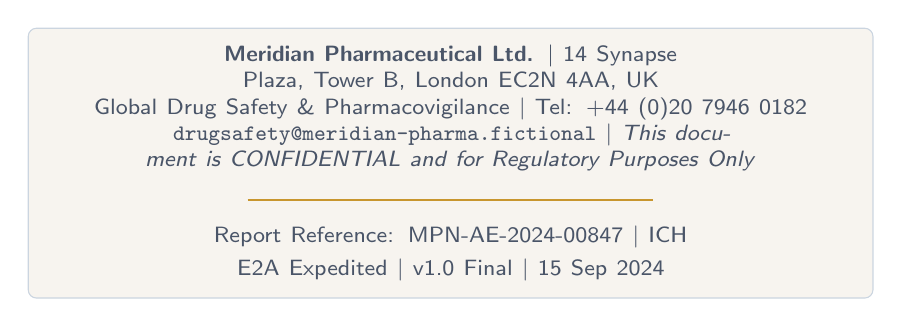
\begin{tikzpicture}
  \node[draw=LightRule, fill=PaperCream, rounded corners=3pt,
        inner sep=6pt, text width=0.85\linewidth, align=center] {
    \footnotesize\color{SlateGray}
    \textbf{Meridian Pharmaceutical Ltd.} \textbar{} 14 Synapse Plaza, Tower B, London EC2N 4AA, UK\\
    Global Drug Safety \& Pharmacovigilance \textbar{} Tel: +44 (0)20 7946 0182\\
    \texttt{drugsafety@meridian-pharma.fictional} \textbar{} \textit{This document is CONFIDENTIAL and for Regulatory Purposes Only}\\[3pt]
    \textcolor{WarmGold}{\rule{0.5\linewidth}{0.8pt}}\\[3pt]
    \footnotesize Report Reference: MPN-AE-2024-00847 \textbar{} ICH E2A Expedited \textbar{} v1.0 Final \textbar{} 15 Sep 2024
  };
\end{tikzpicture}
\end{center}

\end{document}
